%
% Modified by Megan Patnott
% Last Change: Jan 18, 2013
%
%%%%%%%%%%%%%%%%%%%%%%%%%%%%%%%%%%%%%%%%%%%%%%%%%%%%%%%%%%%%%%%%%%%%%%%%
%
% Modified by Sameer Vijay
% Last Change: Wed Jul 27 2005 13:00 CEST
%
%%%%%%%%%%%%%%%%%%%%%%%%%%%%%%%%%%%%%%%%%%%%%%%%%%%%%%%%%%%%%%%%%%%%%%%%
%
% Sample Notre Dame Thesis/Dissertation
% Using Donald Peterson's ndthesis classfile
%
% Written by Jeff Squyres and Don Peterson
%
% Provided by the Information Technology Committee of
%   the Graduate Student Union
%   http://www.gsu.nd.edu/
%
% Nothing in this document is serious except the format.  :-)
%
% If you have any suggestions, comments, questions, please send e-mail
% to: ndthesis@gsu.nd.edu
%
%%%%%%%%%%%%%%%%%%%%%%%%%%%%%%%%%%%%%%%%%%%%%%%%%%%%%%%%%%%%%%%%%%%%%%%%

%
% Chapter 2
%

\chapter{DEVELOPMENT OF METHODS}
\label{chap:development}
This chapter describes the detailed mathematical development of the three real-space methods: Shifted Potential (SP), Gradient Shifted Force (GSF), and Taylor Shifted Force (TSF) for computing electrostatic interactions between point multipoles in molecular simulations. We generalize Wolf's shfited potential for charge-charge interaction to develop multipolar SP method for dipoles and quadrupoles. We also extend original Damped Shifted Force (DSF) method for charge-charge interaction to develop Gradient Shifted Force (GSF) and Taylor Shifted Force (TSF) methods for higher order multipoles. Finally I report the lattice energy constants for different dipolar and quadrupolar crystals evaluated using the newly developed real-space methods and compare with analytical result.

\section{Introduction}
There has been increasing interest in real-space methods for
calculating electrostatic interactions in computer simulations of
condensed molecular systems \cite{Wolf99,Zahn02,Kast03,Beck05,Ma05,Gezelter06,Chen04,Chen06,Rodgers06,Denesyuk08,Izvekov08}
The simplest of these techniques was developed by Wolf {\it et al.}
in their work towards an $\mathcal{O}(N)$ Coulombic sum.\cite{Wolf99}
For systems of point charges, Zahn {\it et al.} extended the Wolf
approach by adding a force-shifting term to the enhanced damped
Coulomb potential.\cite{Zahn02,Kast03} Fennell and Gezelter showed
that the simple damped shifted force (DSF) potential can give nearly
quantitative agreement with smooth particle mesh Ewald
(SPME)\cite{Essmann95} configurational energy differences as well as
atomic force and molecular torque vectors.\cite{Gezelter06}

The computational efficiency and the accuracy of the DSF method are
surprisingly good, particularly for systems with uniform charge
density. Additionally, dielectric constants obtained using DSF and
similar methods where the force vanishes at $r_{c}$ are
essentially quantitative.\cite{Izvekov08} The DSF and other
related methods have now been widely investigated,\cite{Hansen12}
and DSF is now used routinely in a diverse set of chemical
environments.\cite{Shi13,McCann13,Kannam13,Forrest12,English08,Louden13,Tokumasu13}
DSF electrostatics provides a compromise between the computational
speed of real-space cutoffs and the accuracy of fully-periodic Ewald
treatments.

One common feature of many coarse-graining approaches, which treat
entire molecular subsystems as a single rigid body, is simplification
of the electrostatic interactions between these bodies so that fewer
site-site interactions are required to compute configurational
energies. To do this, the interactions between coarse-grained sites
are typically taken to be point
multipoles.\cite{Golubkov06,Orsi10,Orsi11}

Water, in particular, has been modeled recently with point multipoles
up to octupolar
order.\cite{Chowdhuri06,Te10rt,Te10ys,Te10vn} For
maximum efficiency, these models require the use of an approximate
multipole expansion as the exact multipole expansion can become quite
expensive (particularly when handled via the Ewald
sum).\cite{Ichiye06} Point multipoles and multipole
polarizability have also been utilized in the AMOEBA water model and
related force fields.\cite{Ponder10,schnieders07,Ren11}

Higher-order multipoles present a peculiar issue for molecular
dynamics. Multipolar interactions are inherently short-ranged, and
should not need the relatively expensive Ewald treatment.  However,
real-space cutoff methods are normally applied in an orientation-blind
fashion so multipoles which leave and then re-enter a cutoff sphere in
a different orientation can cause energy discontinuities.

This chapter outlines an extension of the original DSF electrostatic
kernel to point multipoles.  We describe three distinct real-space
interaction models for higher-order multipoles based on truncated
Taylor expansions that are carried out at the cutoff radius.  We are
calling these models {\bf Taylor-shifted} (TSF), {\bf
  gradient-shifted} (GSF) and {\bf shifted potential} (SP)
electrostatics.  Because of differences in the initial assumptions,
the two methods yield related, but distinct expressions for energies,
forces, and torques.

In this chapter we outline the new methodology and give functional forms
for the energies, forces, and torques up to quadrupole-quadrupole
order.  We also compare the new methods to analytic energy constants
for periodic arrays of point multipoles. In the following chapter, we
provide numerical comparisons to Ewald-based electrostatics in common
simulation environments.
\section{Methodology}
An efficient real-space electrostatic method involves the use of a
pair-wise functional form,
\begin{equation}
U = \sum_i \sum_{j>i} U_\mathrm{pair}(\mathbf{r}_{ij}, \mathsf{A}_i, \mathsf{B}_j) +
\sum_i U_i^\mathrm{self}
\end{equation}
that is short-ranged and easily truncated at a cutoff radius,
\begin{equation}
  U_\mathrm{pair}(\mathbf{r}_{ij},\mathsf{A}_i, \mathsf{B}_j) = \left\{
\begin{array}{ll}
U_\mathrm{approx} (\mathbf{r}_{ij}, \mathsf{A}_i, \mathsf{B}_j) & \quad \left| \mathbf{r}_{ij} \right| \le r_c \\
0 & \quad \left| \mathbf{r}_{ij} \right|  > r_c ,
\end{array}
\right.
\end{equation}
along with an easily computed self-interaction term ($\sum_i
U_i^\mathrm{self}$) which scales linearly with the number of
particles.  Here $\mathsf{A}_i$ and $\mathsf{B}_j$ represent orientational
coordinates of the two sites (expressed as rotation matrices), and $\mathbf{r}_{ij}$ is the vector
between the two sites.  The computational efficiency, energy
conservation, and even some physical properties of a simulation can
depend dramatically on how the $U_\mathrm{approx}$ function behaves at
the cutoff radius. The goal of any approximation method should be to
mimic the real behavior of the electrostatic interactions as closely
as possible without sacrificing the near-linear scaling of a cutoff
method.

\subsection{Self-neutralization, damping, and force-shifting}
The DSF and Wolf methods operate by neutralizing the total charge
contained within the cutoff sphere surrounding each particle.  This is
accomplished by shifting the potential functions to generate image
charges on the surface of the cutoff sphere for each pair interaction
computed within $r_c$. Damping using a complementary error function is
applied to the potential to accelerate convergence. The interaction
for a pair of charges ($C_i$ and $C_j$) in the DSF method,
\begin{eqnarray}
U_\mathrm{DSF}(r_{ij}) &=&  C_i C_j \left[
\frac{\mathrm{erfc}\left(\alpha r_{ij}\right)}{r_{ij}} 
- \frac{\mathrm{erfc}\left(\alpha r_c\right)}{r_c} \right.\nonumber \\
& & + \left. \left(\frac{\mathrm{erfc}\left(\alpha r_c\right)}{r_c^2} 
+ \frac{2\alpha}{\pi^{1/2}}
\frac{\exp\left(-\alpha^2r_c^2\right)}{r_c}
\right)\left(r_{ij}-r_c\right)\ \right] 
\label{eq:DSFPot}
\end{eqnarray}
where $\alpha$ is the adjustable damping parameter.  Note that in this
potential and in all electrostatic quantities that follow, the
standard $1/4 \pi \epsilon_{0}$ has been omitted for clarity.

To insure net charge neutrality within each cutoff sphere, an
additional ``self'' term is added to the potential. This term is
constant (as long as the charges and cutoff radius do not change), and
exists outside the normal pair-loop for molecular simulations.  It can
be thought of as a contribution from a charge opposite in sign, but
equal in magnitude, to the central charge, which has been spread out
over the surface of the cutoff sphere.  A portion of the self term is
identical to the self term in the Ewald summation, and comes from the
utilization of the complimentary error function for electrostatic
damping.\cite{deLeeuw80,Wolf99} There have also been recent efforts to
extend the Wolf self-neutralization method to zero out the dipole and
higher order multipoles contained within the cutoff
sphere.\cite{Fukuda11,Fukuda12,Fukuda13}

In this work, we extend the idea of self-neutralization for the point
multipoles by insuring net charge-neutrality and net-zero moments
within each cutoff sphere.  In Figure \ref{fig:shiftedMultipoles}, point dipole 
$\mathbf{D}_i$ at the center site $i$ is interacting with point dipole
$\mathbf{D}_j$ and point quadrupole  $\mathsf{Q}_k$.  The
self-neutralization scheme for point multipoles involves projecting
opposing multipoles for sites $j$ and $k$ on the surface of the cutoff
sphere.  There are also significant modifications made to make the
forces and torques go smoothly to zero at the cutoff distance.

\begin{figure}[tpb]
  \begin{center}
    \centerline{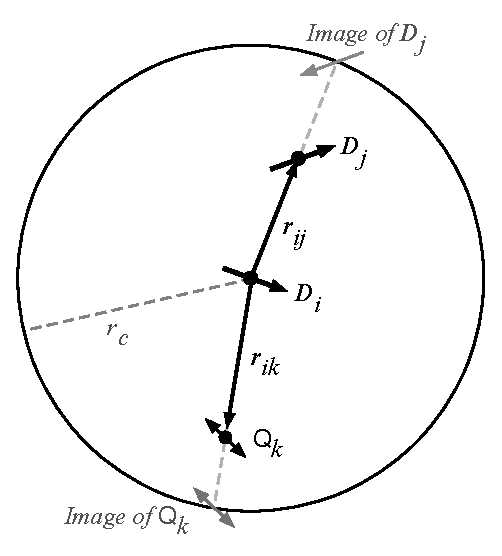
\includegraphics[scale=0.8]{SM.eps}}
    \caption{Reversed multipoles are projected onto the surface of the
  cutoff sphere. The forces, torques, and potential are then smoothly
  shifted to zero as the sites leave the cutoff region.}
    \label{fig:shiftedMultipoles}
  \end{center}
\end{figure}

As in the point-charge approach, there is an additional contribution
from self-neutralization of site $i$.  The self term for multipoles is
described in section \ref{sec:selfTerm}.

\subsection{The multipole expansion}

Consider two discrete rigid collections of point charges, denoted as objects
$a$ and $b$.  In the following, we assume that the two objects
interact via electrostatics only and describe those interactions in
terms of a standard multipole expansion.  Putting the origin of the
coordinate system at the center of mass of $a$, we use vectors
$\mathbf{r}_k$ to denote the positions of all charges $q_k$ in 
$a$.  Then the electrostatic potential of object $a$ at
$\mathbf{r}$ is given by
\begin{equation}
\phi_a(\mathbf r) = 
 \sum_{k \, \text{in } a} \frac{q_k}{\lvert \mathbf{r} - \mathbf{r}_k \rvert}.
\end{equation}
The Taylor expansion in $r$ can be written using an implied summation
notation.  Here Greek indices are used to indicate space coordinates
($x$, $y$, $z$) and the subscripts $k$ and $j$ are reserved for
labeling specific sites for charges in $a$ and $b$ respectively.  The
Taylor expansion,
\begin{equation}
 \frac{1}{\lvert \mathbf{r} - \mathbf{r}_k \rvert} = 
\left( 1
-  r_{k\alpha} \frac{\partial}{\partial r_{\alpha}} 
+ \frac{1}{2}  r_{k\alpha} r_{k\beta} \frac{\partial^2}{\partial r_{\alpha} \partial r_{\beta}} +\dots 
\right)
\frac{1}{r}  ,
\end{equation}
can then be used to express the electrostatic potential on $a$ in
terms of multipole operators,
\begin{equation}
\phi_a(\mathbf{r}) =M_a \frac{1}{r} 
\end{equation}
where
\begin{equation}
M_a = C_a - D_{a\alpha} \frac{\partial}{\partial r_{\alpha}} 
+  Q_{a\alpha\beta}
 \frac{\partial^2}{\partial r_{\alpha} \partial r_{\beta}} + \dots
\end{equation}
Here, the point charge, dipole, and quadrupole for object $a$ are
given by $C_a$, $\mathbf{D}_a$, and $\mathsf{Q}_a$, respectively.  These are the primitive multipoles
which can be expressed as a distribution of charges,
\begin{align}
C_a =&\sum_{k \, \text{in }a} q_k , \label{eq:charge} \\
D_{a\alpha} =&\sum_{k \, \text{in }a} q_k r_{k\alpha}, \label{eq:dipole}\\
Q_{a\alpha\beta} =& \frac{1}{2} \sum_{k \, \text{in }  a} q_k
r_{k\alpha}  r_{k\beta} . \label{eq:quadrupole}
\end{align}
Note that the definition of the primitive quadrupole here differs from
the standard traceless form, and contains an additional Taylor-series
based factor of $1/2$.  We are essentially treating the mass
distribution with higher priority; the moment of inertia tensor,
$\mathsf I$, is diagonalized to obtain body-fixed
axes, and the charge distribution may result in a quadrupole tensor
that is not necessarily diagonal in the body frame.  Additional
reasons for utilizing the primitive quadrupole are discussed in
section \ref{sec:damped}.

It is convenient to locate charges $q_j$ relative to the center of mass of  $b$.  Then with $\bf{r}$ pointing from
the center of mass of $a$ to the center of mass of $b$ ($\mathbf{r}=\mathbf{r}_b - \mathbf{r}_a $), the interaction energy is given by
\begin{equation}
U_{ab}(r)
= M_a \sum_{j \, \text{in } b} \frac {q_j}{\vert \mathbf{r}+\mathbf{r}_j \vert} .
\end{equation}
This can also be expanded as a Taylor series in $r$.  Using a notation
similar to before to define the multipoles in object  $b$,
\begin{equation}
M_b = C_b + D_{b\alpha} \frac{\partial}{\partial r_{\alpha}} 
+   Q_{b\alpha\beta}
 \frac{\partial^2}{\partial r_{\alpha} \partial r_{\beta}} + \dots
\end{equation}
we arrive at the multipole expression for the total interaction energy.
\begin{equation}
U_{ab}(r)=M_a M_b \frac{1}{r}  \label{kernel}.
\end{equation}
This form has the benefit of separating out the energies of
interaction into contributions from the charge, dipole, and quadrupole
of $a$ interacting with the same types of multipoles in $b$.

\subsection{Damped Coulomb interactions}
\label{sec:damped}
In the standard multipole expansion, one typically uses the bare
Coulomb potential, with radial dependence $1/r$, as shown in
Eq.~(\ref{kernel}).  It is also quite common to use a damped Coulomb
interaction, which results from replacing point charges with Gaussian
distributions of charge with width $\alpha$.  In damped multipole
electrostatics, the kernel ($1/r$) of the expansion is replaced with
the function:
\begin{equation}
B_0(r)=\frac{\text{erfc}(\alpha r)}{r} = \frac{2}{\sqrt{\pi}r}
\int_{\alpha r}^{\infty} \text{e}^{-s^2} ds .
\end{equation}
We develop equations below using the function $f(r)$ to represent
either $1/r$ or $B_0(r)$, and all of the techniques can be applied to
bare or damped Coulomb kernels (or any other function) as long as
derivatives of these functions are known.  Smith's convenient
functions $B_l(r)$, which are used for derivatives of the damped
kernel, are summarized in Appendix~\ref{SmithFunc} (N.B. there is one important
distinction between the two kernels, which is the behavior of
$\nabla^2 \frac{1}{r}$ compared with $\nabla^2 B_0(r)$.  The former is
zero everywhere except for a delta function evaluated at the origin.
The latter also has delta function behavior, but is non-zero for $r
\neq 0$.  Thus the standard justification for using a traceless
quadrupole tensor fails for the damped case.)

The main goal of this work is to smoothly cut off the interaction
energy as well as forces and torques as $r\rightarrow r_c$.  To
describe how this goal may be met, we use two examples, charge-charge
and charge-dipole, using the bare Coulomb kernel, $f(r)=1/r$, to
explain the idea.
\subsection{Shifted-force methods}
In the shifted-force approximation, the interaction energy for two
charges $C_a$ and $C_b$ separated by a distance $r$ is
written:
\begin{equation}
U_{C_aC_b}(r)= C_a C_b
\left({ \frac{1}{r} - \frac{1}{r_c} + (r - r_c) \frac{1}{r_c^2}  }
\right) .
\end{equation}
Two shifting terms appear in this equations, one from the
neutralization procedure ($-1/r_c$), and one that causes the first
derivative to vanish at the cutoff radius.

Since one derivative of the interaction energy is needed for the
force, the minimal perturbation is a term linear in $(r-r_c)$ in the
interaction energy, that is:
\begin{equation}
\frac{d\,}{dr} 
\left( {\frac{1}{r} - \frac{1}{r_c} + (r - r_c) \frac{1}{r_c^2}  }
\right) = \left(- \frac{1}{r^2} + \frac{1}{r_c^2} 
\right) .
\end{equation}
which clearly vanishes as the $r$ approaches the cutoff radius. There
are a number of ways to generalize this derivative shift for
higher-order multipoles.  Below, we present two methods, one based on
higher-order Taylor series for $r$ near $r_c$, and the other based on
linear shift of the kernel gradients at the cutoff itself.

\subsection{Taylor-shifted force (TSF) electrostatics}
In the Taylor-shifted force (TSF) method, the procedure that we follow
is based on a Taylor expansion containing the same number of
derivatives required for each force term to vanish at the cutoff.  For
example, the quadrupole-quadrupole interaction energy requires four
derivatives of the kernel, and the force requires one additional
derivative. For quadrupole-quadrupole interactions, we therefore
require shifted energy expressions that include up to $(r-r_c)^5$ so
that all energies, forces, and torques are zero as $r \rightarrow
r_c$. In each case, we subtract off a function $f_n^{\text{shift}}(r)$
from the kernel $f(r)=1/r$.  The subscript $n$ indicates the number of
derivatives to be taken when deriving a given multipole energy.  We
choose a function with guaranteed smooth derivatives -- a truncated
Taylor series of the function $f(r)$, e.g.,
%
\begin{equation}
f_n^{\text{shift}}(r)=\sum_{m=0}^{n+1} \frac {(r-r_c)^m}{m!} f^{(m)}(r_c)  .
\end{equation}
%
The combination of $f(r)$ with the shifted function is denoted $f_n(r)=f(r)-f_n^{\text{shift}}(r)$.
Thus, for $f(r)=1/r$, we find
%
\begin{equation}
f_1(r)=\frac{1}{r}- \frac{1}{r_c} + (r - r_c) \frac{1}{r_c^2} - \frac{(r-r_c)^2}{r_c^3} .
\end{equation}
%
Continuing with the example of a charge $a$ interacting with a
dipole $b$, we write
%
\begin{equation}
U_{C_a\mathbf{D}_b}(r)=
C_a D_{b\alpha}  \frac {\partial f_1(r) }{\partial r_\alpha} 
= C_a D_{b\alpha}
\frac {r_\alpha}{r} \frac {\partial f_1(r)}{\partial r} .
\end{equation}
%
The force that dipole  $ b$ exerts on charge $a$ is
%
\begin{equation}
F_{C_a \mathbf{D}_b \beta} = C_a D_{b \alpha}
\left[ \frac{\delta_{\alpha\beta}}{r} \frac {\partial}{\partial r} + 
\frac{r_\alpha r_\beta}{r^2}
\left( -\frac{1}{r} \frac {\partial} {\partial r} 
+ \frac {\partial ^2} {\partial r^2} \right) \right] f_1(r) .
\end{equation}
%
For undamped coulombic interactions, $f(r)=1/r$, we find
%
\begin{equation}
F_{C_a \mathbf{D}_b \beta} =
\frac{C_a D_{b\beta}}{r}
\left[  -\frac{1}{r^2}+\frac{1}{r_c^2}-\frac{2(r-r_c)}{r_c^3} \right] 
+C_a D_{b \alpha}r_\alpha r_\beta 
\left[ \frac{3}{r^5}-\frac{3}{r^3r_c^2} \right] .
\end{equation}
%
This expansion shows the expected $1/r^3$ dependence of the force.  

In general, we can write
%
\begin{equation}
U^{\text{TSF}}= (\text{prefactor}) (\text{derivatives}) f_n(r)
\label{generic}
\end{equation}
%
with $n=0$ for charge-charge, $n=1$ for charge-dipole, $n=2$ for
charge-quadrupole and dipole-dipole, $n=3$ for dipole-quadrupole, and
$n=4$ for quadrupole-quadrupole.  For example, in
quadrupole-quadrupole interactions for which the $\text{prefactor}$ is
$Q_{a \alpha\beta}Q_{b \gamma\delta}$, the derivatives are
$\partial^4/\partial r_\alpha \partial r_\beta \partial
r_\gamma \partial r_\delta$, with implied summation combining the
space indices.  Appendix \ref{radialTSF} contains details on the
radial functions.

In the formulas presented in the tables below, the placeholder
function $f(r)$ is used to represent the electrostatic kernel (either
damped or undamped).  The main functions that go into the force and
torque terms, $g_n(r), h_n(r), s_n(r), \mathrm{~and~} t_n(r)$ are
successive derivatives of the shifted electrostatic kernel, $f_n(r)$
of the same index $n$.  The algebra required to evaluate energies,
forces and torques is somewhat tedious, so only the final forms are
presented in Tables~\ref{tab:tableenergy} and \ref{tab:tableFORCE}.
One of the principal findings of our work is that the individual
orientational contributions to the various multipole-multipole
interactions must be treated with distinct radial functions, but each
of these contributions is independently force shifted at the cutoff
radius.  
\subsection{Gradient-shifted force (GSF) electrostatics}
The second, and conceptually simpler approach to force-shifting
maintains only the linear $(r-r_c)$ term in the truncated Taylor
expansion, and has a similar interaction energy for all multipole
orders:
\begin{equation}
U^{\text{GSF}} = \sum \left[ U(\mathbf{r}, \mathsf{A}, \mathsf{B}) -
U(r_c \hat{\mathbf{r}},\mathsf{A}, \mathsf{B}) - (r-r_c)
\hat{\mathbf{r}} \cdot \nabla U(r_c \hat{\mathbf{r}},\mathsf{A}, \mathsf{B}) \right]
\label{generic2}
\end{equation}
where $\hat{\mathbf{r}}$ is the unit vector pointing between the two
multipoles, and the sum describes a separate force-shifting that is
applied to each orientational contribution to the energy.  Both the
potential and the gradient for force shifting are evaluated for an
image multipole projected onto the surface of the cutoff sphere (see
fig \ref{fig:shiftedMultipoles}).  The image multipole retains the
orientation (rotation matrix $\mathsf{B}$) of the interacting multipole.  No
higher order terms $(r-r_c)^n$ appear.  The primary difference between
the TSF and GSF methods is the stage at which the Taylor Series is
applied; in the Taylor-shifted approach, it is applied to the kernel
itself.  In the Gradient-shifted approach, it is applied to individual
radial interaction terms in the multipole expansion.  Energies from
this method thus have the general form:
\begin{equation}
U= \sum  (\text{angular factor}) (\text{radial factor}).
\label{generic3}
\end{equation}

Functional forms for both methods (TSF and GSF) can both be summarized
using the form of Eq.~(\ref{generic3}).  The basic forms for the
energy, force, and torque expressions are tabulated for both shifting
approaches below -- for each separate orientational contribution, only
the radial factors differ between the two methods.

\subsection{Generalization of the Wolf shifted potential (SP)}
It is also possible to formulate an extension of the Wolf approach for
multipoles by simply projecting the image multipole onto the surface
of the cutoff sphere, and including the interactions with the central
multipole and the image.  This effectively shifts the pair potential
to zero at the cutoff radius,
\begin{equation}
U^{\text{SP}} = \sum \left[ U(\mathbf{r}, \mathsf{A}, \mathsf{B}) -
U(r_c \hat{\mathbf{r}},\mathsf{A}, \mathsf{B}) \right]
\label{eq:SP}
\end{equation}
independent of the orientations of the two multipoles.  The sum again
describes separate potential shifting that is applied to each
orientational contribution to the energy.
 
The shifted potential (SP) method is a simple truncation of the GSF
method for each orientational contribution, leaving out the $(r-r_c)$
terms that multiply the gradient. Functional forms for the
shifted-potential (SP) method can also be summarized using the form of
Eq.~\ref{generic3}.  The energy, force, and torque expressions are
tabulated below for all three methods. As in the GSF and TSF methods,
for each separate orientational contribution, only the radial factors
differ between the SP, GSF, and TSF methods.


\subsection{\label{sec:level2}Body and space axes}
Although objects $a$ and $b$ rotate during a molecular
dynamics (MD) simulation, their multipole tensors remain fixed in
body-frame coordinates. While deriving force and torque expressions,
it is therefore convenient to write the energies, forces, and torques
in intermediate forms involving the vectors of the rotation matrices.
We denote body axes for objects $a$ and $b$ using unit vectors
$\hat{\mathbf{A}}_m$ and $\hat{\mathbf{B}}_m$, respectively, with the index $m=(123)$.
In a typical simulation, the initial axes are obtained by
diagonalizing the moment of inertia tensors for the objects.  (N.B.,
the body axes are generally {\it not} the same as those for which the
quadrupole moment is diagonal.)  The rotation matrices are then
propagated during the simulation.

The rotation matrices $\mathsf {A}$ and $\mathsf {B}$ can be
expressed using these unit vectors:
\begin{eqnarray}
\mathsf {A} = 
\begin{pmatrix}
\hat{\mathbf{A}}_1 \\
\hat{\mathbf{A}}_2 \\
\hat{\mathbf{A}}_3
\end{pmatrix}, \qquad
\mathsf {B} = 
\begin{pmatrix}
\hat{\mathbf{B}}_1 \\
\hat{\mathbf{B}}_2 \\
\hat{\mathbf{B}}_3
\end{pmatrix}
\end{eqnarray}
%
These matrices convert from space-fixed $(xyz)$ to body-fixed $(123)$
coordinates.

Allen and Germano,\cite{Allen06} following earlier work by Price
{\em et al.},\cite{Price84} showed that if the interaction
energies are written explicitly in terms of $\hat{\mathbf{r}}$ and the body
axes ($\hat{\mathbf{A}}_m$, $\hat{\mathbf{B}}_n$) :
%
\begin{equation}
U(r, \{\hat{\mathbf{A}}_m \cdot \hat{\mathbf{r}} \}, 
\{\hat{\mathbf{B}}_n\cdot \hat{\mathbf{r}} \}, 
\{\hat{\mathbf{A}}_m \cdot \hat{\mathbf{B}}_n \}) .
\label{ugeneral}
\end{equation}
%
the forces come out relatively cleanly,
%
\begin{eqnarray}
\mathbf{F}_a &=&-\mathbf{F}_b =  \nabla U = \frac{\partial U}{\partial \mathbf{r}} \nonumber \\   
&=& \frac{\partial U}{\partial r} \hat{\mathbf{r}} 
 + \sum_m \left[ 
\frac{\partial U}{\partial (\hat{\mathbf{A}}_m \cdot \hat{\mathbf{r}})} 
\frac { \partial (\hat{\mathbf{A}}_m \cdot \hat{\mathbf{r}})}{\partial \mathbf{r}} 
+ \frac{\partial U}{\partial (\hat{\mathbf{B}}_m \cdot \hat{\mathbf{r}})} 
\frac { \partial (\hat{\mathbf{B}}_m \cdot \hat{\mathbf{r}})}{\partial \mathbf{r}} 
\right] \label{forceequation}.
\end{eqnarray}

The torques can also be found in a relatively similar
manner,
%
\begin{eqnarray}
\mathbf{\tau}_a =
 \sum_m 
\frac{\partial U}{\partial (\hat{\mathbf{A}}_m \cdot \hat{\mathbf{r}})} 
( \hat{\mathbf{r}} \times \hat{\mathbf{A}}_m )
-\sum_{mn}
\frac{\partial U}{\partial (\hat{\mathbf{A}}_m \cdot \hat{\mathbf{B}}_n)} 
(\hat{\mathbf{A}}_m \times \hat{\mathbf{B}}_n) \\
%
\mathbf{\tau}_b =
 \sum_m 
\frac{\partial U}{\partial (\hat{\mathbf{B}}_m \cdot \hat{\mathbf{r}})} 
( \hat{\mathbf{r}} \times \hat{\mathbf{B}}_m)
+\sum_{mn}
\frac{\partial U}{\partial (\hat{\mathbf{A}}_m \cdot \hat{\mathbf{B}}_n)} 
(\hat{\mathbf{A}}_m \times \hat{\mathbf{B}}_n) .
\end{eqnarray}

Note that our definition of $\mathbf{r}=\mathbf{r}_b - \mathbf{r}_a $
is opposite in sign to that of Allen and Germano.\cite{Allen06}
We also made use of the identities,
%
\begin{align}
\frac { \partial (\hat{\mathbf{A}}_m \cdot \hat{\mathbf{r}})}{\partial \mathbf{r}} 
=& \frac{1}{r} \left(  \hat{\mathbf{A}}_m - (\hat{\mathbf{A}}_m \cdot \hat{\mathbf{r}})\hat{\mathbf{r}}
\right) \\
\frac { \partial (\hat{\mathbf{B}}_m \cdot \hat{\mathbf{r}})}{\partial \mathbf{r}} 
=& \frac{1}{r} \left(  \hat{\mathbf{B}}_m - (\hat{\mathbf{B}}_m \cdot \hat{\mathbf{r}})\hat{\mathbf{r}} 
\right).
\end{align}

Many of the multipole contractions required can be written in one of
three equivalent forms using the unit vectors $\hat{\mathbf{r}}$, $\hat{\mathbf{A}}_m$,
and $\hat{\mathbf{B}}_n$. In the torque expressions, it is useful to have the
angular-dependent terms available in all three fashions, e.g. for the
dipole-dipole contraction:
%
\begin{equation}
 \mathbf{D}_a \cdot \mathbf{D}_b
= D_{a \alpha} D_{b \alpha} =
\sum_{mn} D_{am} \hat{\mathbf{A}}_m \cdot \hat{\mathbf{B}}_n D_{bn}.
\end{equation}
%
The first two forms are written using space coordinates.  The first
form is standard in the chemistry literature, while the second is
expressed using implied summation notation.  The third form shows
explicit sums over body indices and the dot products now indicate
contractions using space indices. 

In computing our force and torque expressions, we carried out most of
the work in body coordinates, and have transformed the expressions
back to space-frame coordinates, which are reported below.  Interested
readers may consult supplemental information of the Ref. \cite{PaperI} for the intermediate body-frame expressions.

\subsection{The Self-Interaction \label{sec:selfTerm}}

In addition to cutoff-sphere neutralization, the Wolf
summation~\cite{Wolf99} and the damped shifted force (DSF)
extension~\cite{Gezelter06} also include self-interactions that
are handled separately from the pairwise interactions between
sites. The self-term is normally calculated via a single loop over all
sites in the system, and is relatively cheap to evaluate. The
self-interaction has contributions from two sources.

First, the neutralization procedure within the cutoff radius requires
a contribution from a charge opposite in sign, but equal in magnitude,
to the central charge, which has been spread out over the surface of
the cutoff sphere.  For a system of undamped charges, the total
self-term is
\begin{equation}
U_\textrm{self} = - \frac{1}{r_c} \sum_{a=1}^N C_a^{2}.
\label{eq:selfTerm}
\end{equation}
The extension of DSF electrostatics to point multipoles requires
treatment of the self-neutralization \textit{and} reciprocal
contributions to the self-interaction for higher order multipoles.  In
this section we give formulae for these interactions up to quadrupolar
order.

The self-neutralization term is computed by taking the {\it
  non-shifted} kernel for each interaction, placing a multipole of
equal magnitude (but opposite in polarization) on the surface of the
cutoff sphere, and averaging over the surface of the cutoff sphere.
Because the self term is carried out as a single sum over sites, the
reciprocal-space portion is identical to half of the self-term
obtained by Smith, and also by Aguado and Madden for the application
of the Ewald sum to multipoles.\cite{Smith82,Smith98,Aguado03} For a
given site which possesses a charge, dipole, and quadrupole, both types
of contribution are given in Table~\ref{tab:tableSelf}.

\begin{table*}
\begin{center}
  \caption{\label{tab:tableSelf} Self-interaction contributions for 
    site ($a$) that has a charge $(C_a)$, dipole
    $(\mathbf{D}_a)$, and quadrupole $(\mathsf{Q}_a)$}.
\begin{ruledtabular}
\begin{tabular}{|l|c|c|c|} \hline
Multipole order & Summed Quantity & Self-neutralization  & Reciprocal \\ \hline
Charge & $C_a^2$ & $-f(r_c)$ & $-\frac{\alpha}{\sqrt{\pi}}$ \\
Dipole & $|\mathbf{D}_a|^2$ & $\frac{1}{3} \left( h(r_c) +
  \frac{2 g(r_c)}{r_c} \right)$ & $-\frac{2 \alpha^3}{3 \sqrt{\pi}}$\\
Quadrupole & $2 \mathsf{Q}_a:\mathsf{Q}_a + \text{Tr}(\mathsf{Q}_a)^2$ &
$- \frac{1}{15} \left( t(r_c)+ \frac{4 s(r_c)}{r_c} \right)$ &
$-\frac{4 \alpha^5}{5 \sqrt{\pi}}$ \\
Charge-Quadrupole & $-2 C_a \text{Tr}(\mathsf{Q}_a)$ & $\frac{1}{3} \left(
  h(r_c) + \frac{2 g(r_c)}{r_c} \right)$& $-\frac{2 \alpha^3}{3 \sqrt{\pi}}$ \\ \hline
\end{tabular}
\end{ruledtabular}
\end{center}
\end{table*}

For sites which simultaneously contain charges and quadrupoles, the
self-interaction includes a cross-interaction between these two
multipole orders.  Symmetry prevents the charge-dipole and
dipole-quadrupole interactions from contributing to the
self-interaction.  The functions that go into the self-neutralization
terms, $g(r), h(r), s(r), \mathrm{~and~} t(r)$ are successive
derivatives of the electrostatic kernel, $f(r)$ (either the undamped
$1/r$ or the damped $B_0(r)=\mathrm{erfc}(\alpha r)/r$ function) that
have been evaluated at the cutoff distance.  For undamped
interactions, $f(r_c) = 1/r_c$, $g(r_c) = -1/r_c^{2}$, and so on.  For
damped interactions, $f(r_c) = B_0(r_c)$, $g(r_c) = B_0'(r_c)$, and so
on.  Appendix \ref{SmithFunc} contains recursion relations that allow
rapid evaluation of these derivatives.

\section{Interaction energies, forces, and torques}
The main result of this chapter is a set of expressions for the
energies, forces and torques (up to quadrupole-quadrupole order) that
work for the Taylor-shifted, gradient-shifted, and shifted potential
approximations.  These expressions were derived using a set of generic
radial functions.  Without using the shifting approximations mentioned
above, some of these radial functions would be identical, and the
expressions coalesce into the familiar forms for unmodified
multipole-multipole interactions.  Table~\ref{tab:tableenergy} maps
between the generic functions and the radial functions derived for the
three methods.  The energy equations are written in terms of lab-frame
representations of the dipoles, quadrupoles, and the unit vector
connecting the two objects,

% Energy in space coordinate form ----------------------------------------------------------------------------------------------
%
%
% u ca cb
%
\begin{align}
U_{C_a C_b}(r)=&
C_a C_b  v_{01}(r)  \label{uchch}
\\
%
% u ca db
%
U_{C_a \mathbf{D}_b}(r)=&
C_a \left( \mathbf{D}_b \cdot \hat{\mathbf{r}} \right)  v_{11}(r)  
 \label{uchdip}
\\
%
% u ca qb
%
U_{C_a \mathsf{Q}_b}(r)=& C_a \Bigl[ \text{Tr}\mathsf{Q}_b
v_{21}(r) + \left( \hat{\mathbf{r}} \cdot \mathsf{Q}_b \cdot
  \hat{\mathbf{r}} \right) v_{22}(r) \Bigr]
\label{uchquad}
\\
%
% u da cb
%
%U_{D_{\bf a}C_{\bf b}}(r)=&
%-\frac{C_{\bf b}}{4\pi \epsilon_0}  
%\left( \mathbf{D}_{\mathbf{a}} \cdot \hat{r} \right)   v_{11}(r) \label{udipch}
%\\
%
% u da db
%
U_{\mathbf{D}_a \mathbf{D}_b}(r)=&
-\Bigr[ \left( \mathbf{D}_a \cdot
\mathbf{D}_b \right)  v_{21}(r)
+\left( \mathbf{D}_a \cdot \hat{\mathbf{r}} \right)
\left( \mathbf{D}_b \cdot \hat{\mathbf{r}} \right)  
v_{22}(r) \Bigr]
\label{udipdip}
\\
%
% u da qb
%
\begin{split}
% 1
U_{\mathbf{D}_a \mathsf{Q}_b}(r) =&
-\Bigl[
\text{Tr}\mathsf{Q}_b
\left( \mathbf{D}_a \cdot \hat{\mathbf{r}} \right)
+2 ( \mathbf{D}_a \cdot
\mathsf{Q}_b \cdot \hat{\mathbf{r}} ) \Bigr] v_{31}(r) \\
% 2
&- \left( \mathbf{D}_a \cdot \hat{\mathbf{r}} \right)
 \left( \hat{\mathbf{r}} \cdot \mathsf{Q}_b \cdot \hat{\mathbf{r}} \right) v_{32}(r)
\label{udipquad}
\end{split}
\\
%
% u qa cb
%
%U_{Q_{\bf a}C_{\bf b}}(r)=&
%\frac{C_{\bf b }}{4\pi \epsilon_0} \Bigl[ \text{Tr}\mathbf{Q}_{\bf a}  v_{21}(r)
%\left( \hat{r} \cdot \mathbf{Q}_{{\mathbf a}} \cdot \hat{r} \right)  v_{22}(r)  \Bigr]
%\label{uquadch}
%\\
%
% u qa db
%
%\begin{split}
%1
%U_{Q_{\bf a}D_{\bf b}}(r)=&
%\frac{1}{4\pi \epsilon_0} \Bigl[
%\text{Tr}\mathbf{Q}_{\mathbf{a}}
%\left(  \mathbf{D}_{\mathbf{b}} \cdot \hat{r} \right)
%+2 ( \mathbf{D}_{\mathbf{b}} \cdot 
%\mathbf{Q}_{\mathbf{a}}  \cdot \hat{r}) \Bigr] v_{31}(r)\\
% 2
%&+\frac{1}{4\pi \epsilon_0}
%\left(  \mathbf{D}_{\mathbf{b}} \cdot \hat{r} \right)
%\left( \hat{r} \cdot \mathbf{Q}_{{\mathbf a}} \cdot \hat{r} \right) v_{32}(r)
%\label{uquaddip}
%\end{split}
%\\
%
% u qa qb
%
\begin{split}
%1
U_{\mathsf{Q}_a \mathsf{Q}_b}(r)=&
\Bigl[
\text{Tr} \mathsf{Q}_a \text{Tr} \mathsf{Q}_b
+2
\mathsf{Q}_a : \mathsf{Q}_b \Bigr] v_{41}(r)
\\
% 2
&+\Bigl[ \text{Tr}\mathsf{Q}_a
 \left( \hat{\mathbf{r}} \cdot 
\mathsf{Q}_b \cdot \hat{\mathbf{r}} \right)
+\text{Tr}\mathsf{Q}_b
\left( \hat{\mathbf{r}} \cdot \mathsf{Q}_a
 \cdot \hat{\mathbf{r}} \right)  +4 (\hat{\mathbf{r}}  \cdot
\mathsf{Q}_a \cdot \mathsf{Q}_b \cdot \hat{\mathbf{r}})
\Bigr] v_{42}(r)
 \\
% 4
&+ 
\left( \hat{\mathbf{r}} \cdot  \mathsf{Q}_a \cdot \hat{\mathbf{r}} \right)
\left( \hat{\mathbf{r}} \cdot \mathsf{Q}_b  \cdot \hat{\mathbf{r}} \right) v_{43}(r).
\label{uquadquad}
\end{split}
\end{align}
%
Note that the energies of multipoles on site $b$ interacting
with those on site $a$ can be obtained by swapping indices
along with the sign of the intersite vector, $\hat{\mathbf{r}}$.

%
%
% TABLE of radial functions  ----------------------------------------------------------------------------------------------------------------
%

\begin{sidewaystable}
  \caption{\label{tab:tableenergy}Radial functions used in the energy
    and torque equations.  The $f, g, h, s, t, \mathrm{and~} u$
    functions used in this table are defined in Appendices
    \ref{radialTSF} and \ref{radialGSF}.  The gradient shifted (GSF)
    functions include the shifted potential (SP)
    contributions (\textit{cf.} Eqs.~\ref{generic2} and
    \ref{eq:SP}).}
\centering
\resizebox{\textwidth}{!}{\begin{tabular}{|c|c|l|l|l|} \hline
Generic&Bare Coulomb&Taylor-Shifted (TSF)&Shifted Potential (SP)&Gradient-Shifted (GSF)
\\ \hline
%
%
%
%Ch-Ch&
$v_{01}(r)$ &
$\frac{1}{r}$ &
$f_0(r)$ &
$f(r)-f(r_c)$ &
SP $-(r-r_c)g(r_c)$
\\
%
%
%
%Ch-Di&
$v_{11}(r)$ &
$-\frac{1}{r^2}$ &
$g_1(r)$ &
$g(r)-g(r_c)$ &
SP $-(r-r_c)h(r_c)$ \\
%
%
%
%Ch-Qu/Di-Di&
$v_{21}(r)$ &
$-\frac{1}{r^3}  $ & 
$\frac{g_2(r)}{r} $ &
$\frac{g(r)}{r}-\frac{g(r_c)}{r_c}$ &
SP $-(r-r_c) \left( -\frac{g(r_c)}{r_c^2} + \frac{h(r_c)}{r_c} \right)$ \\
%
%
%
$v_{22}(r)$ &
$\frac{3}{r^3}  $ &
$\left(-\frac{g_2(r)}{r} + h_2(r) \right)$ &
$\left(-\frac{g(r)}{r}+h(r) \right) -\left(-\frac{g(r_c)}{r_c}+h(r_c) \right)$ 
& SP $-(r-r_c) \left( \frac{g(r_c)}{r_c^2}-\frac{h(r_c)}{r_c}+s(r_c) \right)$\\
%
%
%
%Di-Qu &
$v_{31}(r)$ &
$\frac{3}{r^4}  $ &
$\left(-\frac{g_3(r)}{r^2} + \frac{h_3(r)}{r} \right)$ &
$\left( -\frac{g(r)}{r^2}+\frac{h(r)}{r}\right)-\left(-\frac{g(r_c)}{r_c^2}+\frac{h(r_c)}{r_c} \right)$ 
& SP $-(r-r_c) \left(\frac{2g(r_c)}{r_c^3}-\frac{2h(r_c)}{r_c^2}+\frac{s(r_c)}{r_c} \right)$  \\
% 
%
%
$v_{32}(r)$ &
$-\frac{15}{r^4}  $ &
$\left( \frac{3g_3(r)}{r^2} - \frac{3h_3(r)}{r} + s_3(r) \right)$ &
$\left( \frac{3g(r)}{r^2} - \frac{3h(r)}{r} + s(r) \right)$&
SP $-(r-r_c) \left( \frac{-6g(r_c)}{r_c^3}+\frac{6h(r_c)}{r_c^2}\right.$ \\
&&& $~~~-\left(\frac{3g(r_c)}{r_c^2} - \frac{3h(r_c)}{r_c} + s(r_c)\right)$ & 
$\phantom{SP-(r-r_c)}\left.-\frac{3s(r_c)}{r_c}+t(r_c) \right)$\\
%
%
%
%Qu-Qu&
$v_{41}(r)$ &
$\frac{3}{r^5} $ &
$\left(-\frac{g_4(r)}{r^3} +\frac{h_4(r)}{r^2} \right) $  &
$\left( -\frac{g(r)}{r^3} + \frac{h(r)}{r^2} \right)- \left(-\frac{g(r_c)}{r_c^3} + \frac{h(r_c)}{r_c^2} \right)$ & 
SP $-(r-r_c) \left( \frac{3g(r_c)}{r_c^4}-\frac{3h(r_c)}{r_c^3}+\frac{s(r_c)}{r_c^2} \right)$ 
\\
% 2
$v_{42}(r)$ &
$- \frac{15}{r^5}   $ &
$\left( \frac{3g_4(r)}{r^3} - \frac{3h_4(r)}{r^2}+\frac{s_4(r)}{r} \right)$ &
$\left( \frac{3g(r)}{r^3} - \frac{3h(r)}{r^2}+\frac{s(r)}{r} \right)$ & 
SP$-(r-r_c) \left(- \frac{9g(r_c)}{r_c^4}+\frac{9h(r_c)}{r_c^3}\right.$  \\
&&& $~~~-\left( \frac{3g(r_c)}{r_c^3} -  \frac{3h(r_c)}{r_c^2}+\frac{s(r_c)}{r_c} \right)$ & 
$\phantom{SP-(r-r_c)}\left. -\frac{4s(r_c)}{r_c^2} + \frac{t(r_c)}{r_c}\right)$\\
% 3
%
%
$v_{43}(r)$ &
$ \frac{105}{r^5}  $ &
$\left(-\frac{15g_4(r)}{r^3}+\frac{15h_4(r)}{r^2}-\frac{6s_4(r)}{r} + t_4(r)\right) $ &
$ \left(-\frac{15g(r)}{r^3} +\frac{15h(r)}{r^2}-\frac{6s(r)}{r}+t(r)\right) $ &
SP $-(r-r_c)\left(\frac{45g(r_c)}{r_c^4}-\frac{45h(r_c)}{r_c^3}\right.$\\
&&& $~~~-\left(-\frac{15g(r_c)}{r_c^3}+\frac{15h(r_c)}{r_c^2}-\frac{6s(r_c)}{r_c}+ t(r_c)\right)$ & 
$\phantom{SP-(r-r_c)}\left.+\frac{21s(r_c)}{r_c^2}-\frac{6t(r_c)}{r_c}+u(r_c) \right)$\\
\hline
\end{tabular}}
\end{sidewaystable}
%
%
% FORCE	 TABLE of radial functions  ----------------------------------------------------------------------------------------------------------------
%

\begin{sidewaystable}
\caption{\label{tab:tableFORCE}Radial functions used in the force
  equations. Gradient shifted (GSF) functions are constructed using the shifted
    potential (SP) functions.  Some of these functions are simple
    modifications of the functions found in Table~\ref{tab:tableenergy}}
\centering
\resizebox{\textwidth}{!}{\begin{tabular}{|c|c|l|l|l|} \hline
Function&Definition&Taylor-Shifted (TSF)& Shifted Potential (SP)
&Gradient-Shifted (GSF)
\\ \hline
%
%
%
$w_a(r)$&
$\frac{d v_{01}}{dr}$&
$g_0(r)$&
$g(r)$&
SP $-g(r_c)$ \\
%
%
$w_b(r)$ &
$\frac{d v_{11}}{dr} - \frac{v_{11}(r)}{r} $&
$\left( -\frac{g_1(r)}{r}+h_1(r) \right)$ &
$h(r) - \frac{v_{11}(r)}{r} $ &
SP $- h(r_c)$ \\
%
$w_c(r)$ &
$\frac{v_{11}(r)}{r}$ &
$\frac{g_1(r)}{r} $ &
$\frac{v_{11}(r)}{r}$&
$\frac{v_{11}(r)}{r}$\\
%
%
$w_d(r)$&
$\frac{d v_{21}}{dr}$&
$\left( -\frac{g_2(r)}{r^2} + \frac{h_2(r)}{r} \right) $ &
$\left( -\frac{g(r)}{r^2} + \frac{h(r)}{r} \right)$ &
SP $-\left( -\frac{g(r_c)}{r_c^2} + \frac{h(r_c)}{r_c} \right) $ \\
%
$w_e(r)$ &
$\frac{v_{22}(r)}{r}$&
$\left(-\frac{g_2(r)}{r^2} + \frac{h_2(r)}{r} \right)$ &
$\frac{v_{22}(r)}{r}$ &
$\frac{v_{22}(r)}{r}$ \\
% 
%
$w_f(r)$&
$\frac{d v_{22}}{dr} - \frac{2v_{22}(r)}{r}$&
$\left( \frac{3g_2(r)}{r^2}-\frac{3h_2(r)}{r}+s_2(r) \right)$ &
  $ \left( \frac{g(r)}{r^2}-\frac{h(r)}{r}+s(r) \right) -\frac{2v_{22}(r)}{r}$&
SP $- \left( \frac{g(r_c)}{r_c^2}-\frac{h(r_c)}{r_c}+s(r_c) \right)$\\
%
$w_g(r)$& 
$\frac{v_{31}(r)}{r}$& 
$ \left( -\frac{g_3(r)}{r^3}+\frac{h_3(r)}{r^2} \right)$& 
$\frac{v_{31}(r)}{r}$&
$\frac{v_{31}(r)}{r}$\\
%
$w_h(r)$ &
$\frac{d v_{31}}{dr} -\frac{v_{31}(r)}{r}$&
$\left(\frac{3g_3(r)}{r^3} -\frac{3h_3(r)}{r^2} +\frac{s_3(r)}{r} \right) $  &
$ \left(\frac{2g(r)}{r^3} -\frac{2h(r)}{r^2} +\frac{s(r)}{r} \right) -\frac{v_{31}(r)}{r}$ &
SP $ - \left(\frac{2g(r_c)}{r_c^3} -\frac{2h(r_c)}{r_c^2} +\frac{s(r_c)}{r_c} \right) $ \\
% 2
$w_i(r)$ &
$\frac{v_{32}(r)}{r}$ &
$\left(\frac{3g_3(r)}{r^3} -\frac{3h_3(r)}{r^2} +\frac{s_3(r)}{r} \right) $  &
$\frac{v_{32}(r)}{r}$&
$\frac{v_{32}(r)}{r}$\\
% 
$w_j(r)$ &
$\frac{d v_{32}}{dr}  - \frac{3v_{32}}{r}$&
$\left(\frac{-15g_3(r)}{r^3} + \frac{15h_3(r)}{r^2} - \frac{6s_3(r)}{r} + t_3(r) \right)  $ &
$\left(\frac{-6g(r)}{r^3} +\frac{6h(r)}{r^2} -\frac{3s(r)}{r} +t(r) \right) -\frac{3v_{32}}{r}$ &
SP $-\left(\frac{-6g(_cr)}{r_c^3} +\frac{6h(r_c)}{r_c^2}
  -\frac{3s(r_c)}{r_c} +t(r_c) \right)$ \\
%
$w_k(r)$ &
$\frac{d v_{41}}{dr} $ &
$\left(\frac{3g_4(r)}{r^4} -\frac{3h_4(r)}{r^3} +\frac{s_4(r)}{r^2}  \right)$ &
$\left(\frac{3g(r)}{r^4} -\frac{3h(r)}{r^3} +\frac{s(r)}{r^2}
\right)$ &
SP $-\left(\frac{3g(r_c)}{r_c^4} -\frac{3h(r_c)}{r_c^3} +\frac{s(r_c)}{r_c^2}  \right)$ \\
%
$w_l(r)$ &
$\frac{d v_{42}}{dr} -\frac{2v_{42}(r)}{r}$ &
$\left(-\frac{15g_4(r)}{r^4} +\frac{15h_4(r)}{r^3} -\frac{6s_4(r)}{r^2} +\frac{t_4(r)}{r} \right)$ &
$\left(-\frac{9g(r)}{r^4} +\frac{9h(r)}{r^3} -\frac{4s(r)}{r^2}
  +\frac{t(r)}{r} \right) -\frac{2v_{42}(r)}{r}$&
SP$-\left(-\frac{9g(r_c)}{r_c^4} +\frac{9h(r_c)}{r_c^3} -\frac{4s(r_c)}{r_c^2} +\frac{t(r_c)}{r_c} \right)$\\
%
$w_m(r)$ &
$\frac{d v_{43}}{dr} -\frac{4v_{43}(r)}{r}$&
$\left(\frac{105g_4(r)}{r^4} - \frac{105h_4(r)}{r^3} \right.$ &
$\left(\frac{45g(r)}{r^4} -\frac{45h(r)}{r^3} +\frac{21s(r)}{r^2}\right.$ &
SP $- \left(\frac{45g(r_c)}{r_c^4} -\frac{45h(r_c)}{r_c^3}\right.$ \\
&& $~~~\left.+ \frac{45s_4(r)}{r^2} - \frac{10t_4(r)}{r} +u_4(r) \right)$
& $~~~\left. -\frac{6t(r)}{r} +u(r) \right) -\frac{4v_{43}(r)}{r}$ &
$\phantom{SP-} \left.+\frac{21s(r_c)}{r_c^2} -\frac{6t(r_c)}{r_c} +u(r_c) \right) $\\ 
%
$w_n(r)$ &
$\frac{v_{42}(r)}{r}$ &
$\left(\frac{3g_4(r)}{r^4} -\frac{3h_4(r)}{r^3} +\frac{s_4(r)}{r^2}  \right)$ &
$\frac{v_{42}(r)}{r}$&
$\frac{v_{42}(r)}{r}$\\
%
$w_o(r)$ &
$\frac{v_{43}(r)}{r}$&
$\left(-\frac{15g_4(r)}{r^4} +\frac{15h_4(r)}{r^3} -\frac{6s_4(r)}{r^2} +\frac{t_4(r)}{r} \right)$ &
$\frac{v_{43}(r)}{r}$&
$\frac{v_{43}(r)}{r}$  \\ \hline
%

\end{tabular}}
\end{sidewaystable}


\subsection{Forces}
The force on object $a$, $\mathbf{F}_a$, due to object
$b$ is the negative of the force on $b$ due to $a$. For
a simple charge-charge interaction, these forces will point along the
$\pm \hat{\mathbf{r}}$ directions, where $\mathbf{r}=\mathbf{r}_b -
\mathbf{r}_a $.  Thus
%
\begin{equation}
F_{a \alpha} = \hat{r}_\alpha \frac{\partial U_{C_a C_b}}{\partial r} 
\quad \text{and} \quad  F_{b \alpha} 
= - \hat{r}_\alpha \frac{\partial U_{C_a C_b}} {\partial r}  .
\end{equation}
%
We list below the force equations written in terms of lab-frame
coordinates.  The radial functions used in the three methods are listed
in Table~\ref{tab:tableFORCE}
%
%SPACE COORDINATES FORCE EQUATIONS
%
% **************************************************************************
% f ca cb
%
\begin{align}
\mathbf{F}_{a {C_a} {C_b}} =&
C_a C_b  w_a(r) \hat{\mathbf{r}} \\
%
%
%
\mathbf{F}_{a {C_a} {\mathbf{D}_b} } =&
C_a \Bigl[
 \left( \hat{\mathbf{r}} \cdot \mathbf{D}_b  \right) 
w_b(r) \hat{\mathbf{r}}  
+ \mathbf{D}_b w_c(r) \Bigr] \\
%
%
%
\mathbf{F}_{a {C_a} {\mathsf{Q}_b}} =&
C_a \Bigr[
\text{Tr}\mathsf{Q}_b w_d(r) \hat{\mathbf{r}}
+ 2  \mathsf{Q}_b \cdot \hat{\mathbf{r}} w_e(r)
 + \left( \hat{\mathbf{r}} \cdot  \mathsf{Q}_b \cdot \hat{\mathbf{r}}
 \right) w_f(r) \hat{\mathbf{r}} \Bigr] \\
%
%
%
% \begin{equation}
% \mathbf{F}_{{\bf a}D_{\bf a}C_{\bf b}} = 
% -C_{\bf{b}} \Bigl[
% \left( \hat{r} \cdot  \mathbf{D}_{\mathbf{a}} \right) w_b(r) \hat{r}
% + \mathbf{D}_{\mathbf{a}} w_c(r) \Bigr]
% \end{equation}
%
%
%
\begin{split}
\mathbf{F}_{a \mathbf{D}_a \mathbf{D}_b} =&
- \mathbf{D}_a \cdot  \mathbf{D}_b w_d(r) \hat{\mathbf{r}}
+ \left( \mathbf{D}_a 
\left( \mathbf{D}_b \cdot \hat{\mathbf{r}} \right)
+ \mathbf{D}_b \left( \mathbf{D}_a  \cdot \hat{\mathbf{r}} \right) \right) w_e(r)\\
% 2
& - \left( \hat{\mathbf{r}} \cdot \mathbf{D}_a \right) 
\left( \hat{\mathbf{r}} \cdot \mathbf{D}_b \right) w_f(r) \hat{\mathbf{r}}
\end{split}\\
%
%
%
\begin{split}
\mathbf{F}_{a \mathbf{D}_a \mathsf{Q}_b} =& - \Bigl[
\text{Tr}\mathsf{Q}_b \mathbf{ D}_a
+2 \mathbf{D}_a \cdot 
\mathsf{Q}_b \Bigr] w_g(r)
 - \Bigl[
\text{Tr}\mathsf{Q}_b
\left( \hat{\mathbf{r}} \cdot  \mathbf{D}_a \right) 
+2 ( \mathbf{D}_a \cdot 
\mathsf{Q}_b \cdot \hat{\mathbf{r}}) \Bigr] w_h(r) \hat{\mathbf{r}}  \\
% 3
& - \Bigl[\mathbf{ D}_a  (\hat{\mathbf{r}} \cdot \mathsf{Q}_b \cdot \hat{\mathbf{r}}) 
+2  (\hat{\mathbf{r}} \cdot \mathbf{D}_a ) (\hat{\mathbf{r}} \cdot \mathsf{Q}_b )  \Bigr]
w_i(r)
% 4
 -
(\hat{\mathbf{r}} \cdot \mathbf{D}_a )
(\hat{\mathbf{r}} \cdot \mathsf{Q}_b \cdot \hat{\mathbf{r}}) w_j(r) \hat{\mathbf{r}} \end{split} \\
%
%
% \begin{equation}
% \mathbf{F}_{{\bf a}Q_{\bf a}C_{\bf b}} = 
% \frac{C_{\bf b }}{4\pi \epsilon_0} \Bigr[
% \text{Tr}\mathbf{Q}_{\bf a} w_d(r) \hat{r}
% + 2  \mathbf{Q}_{{\mathbf a}} \cdot \hat{r} w_e(r)
%  + \left( \hat{r} \cdot  \mathbf{Q}_{{\mathbf a}} \cdot \hat{r} \right) w_f(r) \hat{r} \Bigr]
% \end{equation}
% %
% \begin{equation}
% \begin{split}
% \mathbf{F}_{{\bf a}Q_{\bf a}D_{\bf b}} = 
% &\frac{1}{4\pi \epsilon_0} \Bigl[
% \text{Tr}\mathbf{Q}_{\mathbf{a}} \mathbf{D}_{\mathbf{b}} 
% +2 \mathbf{D}_{\mathbf{b}} \cdot \mathbf{Q}_{\mathbf{a}}  \Bigr] w_g(r)
% % 2
% + \frac{1}{4\pi \epsilon_0} \Bigl[ \text{Tr}\mathbf{Q}_{\mathbf{a}}
% (\hat{r} \cdot  \mathbf{D}_{\mathbf{b}})
% +2 (\mathbf{D}_{\mathbf{b}} \cdot 
% \mathbf{Q}_{\mathbf{a}} \cdot \hat{r}) \Bigr] w_h(r) \hat{r}  \\
% % 3
% &+ \frac{1}{4\pi \epsilon_0} \Bigl[ \mathbf{D}_{\mathbf{b}} 
% (\hat{r} \cdot \mathbf{Q}_{{\mathbf a}} \cdot \hat{r}) 
% +2  (\hat{r} \cdot \mathbf{D}_{\mathbf{b}})
% (\hat{r} \cdot  \mathbf{Q}_{{\mathbf a}} ) \Bigr]   w_i(r)
% % 4
% +\frac{1}{4\pi \epsilon_0} 
% (\hat{r} \cdot \mathbf{D}_{\mathbf{b}}) 
% (\hat{r} \cdot \mathbf{Q}_{{\mathbf a}}  \cdot \hat{r}) w_j(r) \hat{r} 
% \end{split}
% \end{equation}
%
%
%
\begin{split}
\mathbf{F}_{a \mathsf{Q}_a \mathsf{Q}_b} =& 
 \Bigl[
\text{Tr}\mathsf{Q}_a \text{Tr}\mathsf{Q}_b 
+ 2  \mathsf{Q}_a :  \mathsf{Q}_b \Bigr] w_k(r) \hat{\mathbf{r}} \\
% 2
&+ \Bigl[
2\text{Tr}\mathsf{Q}_b  (\hat{\mathbf{r}} \cdot \mathsf{Q}_a )  
+ 2\text{Tr}\mathsf{Q}_a  (\hat{\mathbf{r}} \cdot \mathsf{Q}_b ) 
% 3
+4 (\mathsf{Q}_a  \cdot  \mathsf{Q}_b \cdot \hat{\mathbf{r}})  
+  4(\hat{\mathbf{r}} \cdot \mathsf{Q}_a \cdot \mathsf{Q}_b) \Bigr] w_n(r) \\
% 4
&+  \Bigl[
\text{Tr}\mathsf{Q}_a (\hat{\mathbf{r}} \cdot \mathsf{Q}_b \cdot \hat{\mathbf{r}}) 
+ \text{Tr}\mathsf{Q}_b
(\hat{\mathbf{r}} \cdot \mathsf{Q}_a  \cdot \hat{\mathbf{r}})  
% 5
+4 (\hat{\mathbf{r}} \cdot \mathsf{Q}_a \cdot  
\mathsf{Q}_b   \cdot \hat{\mathbf{r}}) \Bigr] w_l(r) \hat{\mathbf{r}} \\
%
&+ \Bigl[
+ 2 (\hat{\mathbf{r}} \cdot \mathsf{Q}_a )
(\hat{\mathbf{r}} \cdot \mathsf{Q}_b \cdot \hat{\mathbf{r}})
%6
+2 (\hat{\mathbf{r}} \cdot \mathsf{Q}_a \cdot \hat{\mathbf{r}})
(\hat{\mathbf{r}} \cdot \mathsf{Q}_b ) \Bigr] w_o(r) \\
%  7
&+ 
(\hat{\mathbf{r}} \cdot \mathsf{Q}_a  \cdot \hat{\mathbf{r}}) 
(\hat{\mathbf{r}} \cdot \mathsf{Q}_b \cdot \hat{\mathbf{r}}) w_m(r) \hat{\mathbf{r}} \end{split}
\end{align}
Note that the forces for higher multipoles on site $a$
interacting with those of lower order on site $b$ can be
obtained by swapping indices in the expressions above.

%
% Torques SECTION -----------------------------------------------------------------------------------------
\subsection{Torques}

%
The torques for the three methods are given in space-frame
coordinates:
%
%
\begin{align}
\mathbf{\tau}_{b C_a \mathbf{D}_b} =& 
C_a  (\hat{\mathbf{r}} \times  \mathbf{D}_b) v_{11}(r) \\
%
%
%
\mathbf{\tau}_{b C_a \mathsf{Q}_b} =&
2C_a
\hat{\mathbf{r}} \times ( \mathsf{Q}_b \cdot \hat{\mathbf{r}}) v_{22}(r) \\
%
%
%
% \begin{equation}
% \mathbf{\tau}_{{\bf a}D_{\bf a}C_{\bf b}} =  
% -\frac{C_{\bf b}}{4\pi \epsilon_0}  
% (\hat{r} \times \mathbf{D}_{\mathbf{a}})  v_{11}(r) 
% \end{equation}
%
%
%
\mathbf{\tau}_{a \mathbf{D}_a \mathbf{D}_b} =&
 \mathbf{D}_a  \times \mathbf{D}_b v_{21}(r)
% 2
-
(\hat{\mathbf{r}} \times \mathbf{D}_a )
(\hat{\mathbf{r}} \cdot \mathbf{D}_b )  v_{22}(r)\\
%
%
%
% \begin{equation}
% \mathbf{\tau}_{{\bf b}D_{\bf a}D_{\bf b}} = 
% -\frac{1}{4\pi \epsilon_0} \mathbf{D}_{\mathbf {a}} \times \mathbf{D}_{\mathbf{b}} v_{21}(r)
% % 2
% +\frac{1}{4\pi \epsilon_0} 
% (\hat{r} \cdot \mathbf{D}_{\mathbf {a}} )
% (\hat{r} \times \mathbf{D}_{\mathbf {b}} ) v_{22}(r)
% \end{equation}
%
%
%
\mathbf{\tau}_{a \mathbf{D}_a \mathsf{Q}_b} =& 
 \Bigl[
-\text{Tr}\mathsf{Q}_b
(\hat{\mathbf{r}} \times \mathbf{D}_a )
+2 \mathbf{D}_a  \times 
(\mathsf{Q}_b \cdot \hat{\mathbf{r}})
\Bigr] v_{31}(r)
% 3
- (\hat{\mathbf{r}} \times \mathbf{D}_a )
(\hat{\mathbf{r}} \cdot \mathsf{Q}_b \cdot \hat{\mathbf{r}}) v_{32}(r)\\
%
%
%
\mathbf{\tau}_{b \mathbf{D}_a \mathsf{Q}_b} =&
 \Bigl[
+2 ( \mathbf{D}_a \cdot \mathsf{Q}_b ) \times
\hat{\mathbf{r}} 
-2 \mathbf{D}_a  \times 
(\mathsf{Q}_b \cdot \hat{\mathbf{r}})
\Bigr] v_{31}(r)
% 2
+
(\hat{\mathbf{r}} \cdot \mathbf{D}_a)
(\hat{\mathbf{r}} \cdot \mathsf{Q}_b) \times \hat{\mathbf{r}} v_{32}(r)\\
%
%
%
% \begin{equation}
% \mathbf{\tau}_{{\bf a}Q_{\bf a}D_{\bf b}} =
% \frac{1}{4\pi \epsilon_0} \Bigl[
% -2 (\mathbf{D}_{\mathbf{b}}  \cdot \mathbf{Q}_{\mathbf{a}} ) \times \hat{r} 
% +2 \mathbf{D}_{\mathbf{b}}  \times 
% (\mathbf{Q}_{\mathbf{a}}  \cdot \hat{r})
% \Bigr] v_{31}(r)
% % 3
% - \frac{2}{4\pi \epsilon_0}
% (\hat{r} \cdot \mathbf{D}_{\mathbf{b}} )
% (\hat{r} \cdot  \mathbf
% {Q}_{{\mathbf a}}) \times \hat{r} v_{32}(r)
% \end{equation}
%
%
%
% \begin{equation}
% \mathbf{\tau}_{{\bf b}Q_{\bf a}D_{\bf b}} = 
% \frac{1}{4\pi \epsilon_0} \Bigl[
% \text{Tr}\mathbf{Q}_{\mathbf{a}}
% (\hat{r} \times \mathbf{D}_{\mathbf{b}} )
% +2 \mathbf{D}_{\mathbf{b}}  \times
% ( \mathbf{Q}_{\mathbf{a}} \cdot \hat{r}) \Bigr] v_{31}(r)
% % 2
% +\frac{1}{4\pi \epsilon_0}
% (\hat{r} \times \mathbf{D}_{\mathbf{b}} )
% (\hat{r} \cdot \mathbf{Q}_{{\mathbf a}} \cdot \hat{r}) v_{32}(r)
% \end{equation}
%
%
%
\begin{split}
\mathbf{\tau}_{a \mathsf{Q}_a \mathsf{Q}_b} =&
-4 
\mathsf{Q}_a \times \mathsf{Q}_b
v_{41}(r) \\
% 2
&+ 
\Bigl[-2\text{Tr}\mathsf{Q}_b
(\hat{\mathbf{r}} \cdot \mathsf{Q}_a ) \times \hat{\mathbf{r}}
+4 \hat{\mathbf{r}} \times 
( \mathsf{Q}_a \cdot \mathsf{Q}_b \cdot \hat{\mathbf{r}}) 
% 3
-4 (\hat{\mathbf{r}} \cdot \mathsf{Q}_a )\times 
( \mathsf{Q}_b \cdot \hat{\mathbf{r}} ) \Bigr] v_{42}(r) \\
% 4
&+ 2
\hat{\mathbf{r}} \times ( \mathsf{Q}_a \cdot \hat{\mathbf{r}})
(\hat{\mathbf{r}} \cdot \mathsf{Q}_b \cdot \hat{\mathbf{r}}) v_{43}(r) \end{split}\\
%
%
%
\begin{split}
\mathbf{\tau}_{b \mathsf{Q}_a \mathsf{Q}_b} =  
&4
\mathsf{Q}_a \times \mathsf{Q}_b v_{41}(r) \\
% 2
&+  \Bigl[- 2\text{Tr}\mathsf{Q}_a
(\hat{\mathbf{r}} \cdot \mathsf{Q}_b ) \times \hat{\mathbf{r}}
-4  (\hat{\mathbf{r}} \cdot \mathsf{Q}_a \cdot 
\mathsf{Q}_b ) \times
\hat{\mathbf{r}} 
+4 ( \hat{\mathbf{r}} \cdot \mathsf{Q}_a ) \times 
( \mathsf{Q}_b \cdot \hat{\mathbf{r}})
\Bigr] v_{42}(r) \\
% 4
&+2
(\hat{\mathbf{r}} \cdot \mathsf{Q}_a \cdot \hat{\mathbf{r}})
\hat{\mathbf{r}} \times ( \mathsf{Q}_b \cdot \hat{\mathbf{r}}) v_{43}(r)\end{split}
\end{align}
%
Here, we have defined the matrix cross product in an identical form
as in Ref. \cite{Smith98}:
\begin{equation}
\left[\mathsf{A} \times \mathsf{B}\right]_\alpha = \sum_\beta
\left[\mathsf{A}_{\alpha+1,\beta} \mathsf{B}_{\alpha+2,\beta}
  -\mathsf{A}_{\alpha+2,\beta} \mathsf{B}_{\alpha+1,\beta} 
\right]
\label{eq:matrixCross}
\end{equation}
where $\alpha+1$ and $\alpha+2$ are regarded as cyclic
permuations of the matrix indices.

All of the radial functions required for torques are identical with
the radial functions previously computed for the interaction energies.
These are tabulated for all three methods in Table~\ref{tab:tableenergy}.  The torques for higher multipoles on site
$a$ interacting with those of lower order on site
$b$ can be obtained by swapping indices in the expressions
above.
\section{Comparison to known multipolar energies}

To understand how these new real-space multipole methods behave in
computer simulations, it is vital to test against established methods
for computing electrostatic interactions in periodic systems, and to
evaluate the size and sources of any errors that arise from the
real-space cutoffs. In this chapter we test SP, TSF, and GSF
electrostatics against analytical methods for computing the energies
of ordered multipolar arrays.  In the following chapter, we test the new
methods against the multipolar Ewald sum for computing the energies,
forces and torques for a wide range of typical condensed-phase
(disordered) systems.

Because long-range electrostatic effects can be significant in
crystalline materials, ordered multipolar arrays present one of the
biggest challenges for real-space cutoff methods.  The dipolar
analogues to the Madelung constants were first worked out by Sauer,
who computed the energies of ordered dipole arrays of zero
magnetization and obtained a number of these constants.\cite{Sauer}
This theory was developed more completely by Luttinger and
Tisza\cite{LT,LT2} who tabulated energy constants for the Sauer arrays
and other periodic structures.  

To test the new electrostatic methods, we have constructed very large,
$N=$ 16,000~(bcc) arrays of dipoles in the orientations described in
Ref. \cite{LT}.  These structures include ``A'' lattices with
nearest neighbor chains of antiparallel dipoles, as well as ``B''
lattices with nearest neighbor strings of antiparallel dipoles if the
dipoles are contained in a plane perpendicular to the dipole direction
that passes through the dipole.  We have also studied the minimum
energy structure for the BCC lattice that was found by Luttinger \&
Tisza.  The total electrostatic energy density for any of the arrays
is given by:
\begin{equation}
  E = C N^2 \mu^2
\end{equation}
where $C$ is the energy constant (equivalent to the Madelung
constant), $N$ is the number of dipoles per unit volume, and $\mu$ is
the strength of the dipole. Energy constants (converged to 1 part in
$10^9$) are given in the supplemental information Ref. \cite{PaperI}.
\begin{figure}[tpb]
  \begin{center}
    \centerline{\includegraphics[width = \linewidth]{Dipoles_rcut_threeAlpha.pdf}}
    \caption{Convergence of the lattice energy constants as a function of
  cutoff radius (normalized by the lattice constant, $a$) for the new
  real-space methods.  Three dipolar crystal structures were sampled,
  and the analytic energy constants for the three lattices are
  indicated with grey dashed lines.  The left panel shows results for
  the undamped kernel ($1/r$), while the damped kernel, $B_0(r)$ was
  used in the center and right panels.}
\label{fig:Dipoles_rCut}
  \end{center}
\end{figure}

For the purposes of testing the energy expressions and the
self-neutralization schemes, the primary quantity of interest is the
analytic energy constant for the perfect arrays.  Convergence to these
constants are shown as a function of the cutoff radius, $r_c$, for
three different values of the damping coefficient, $\alpha$ in
Fig.\ref{fig:Dipoles_rCut}.  We have simultaneously tested a hard
cutoff (where the kernel is simply truncated at the cutoff radius) in
addition to the three new methods.

The hard cutoff exhibits oscillations around the analytic energy
constants, and converges to incorrect energies when the complementary
error function damping kernel is used.  The shifted potential (SP)
converges to the correct energy smoothly by $r_c = 4.5 a$ even for the
undamped case. This indicates that the shifting and the correction
provided by the self term are required for obtaining accurate
energies. The Taylor-shifted force (TSF) approximation appears to
perturb the potential too much inside the cutoff region to provide
accurate measures of the energy constants.  GSF is a compromise,
converging to the correct energies within $r_c = 6 a$.

{\it Quadrupolar} analogues to the Madelung constants were first
worked out by Nagai and Nakamura who computed the energies of selected
quadrupole arrays based on extensions to the Luttinger and Tisza
approach.\cite{Nagai60,Nagai63} 

In analogy to the dipolar arrays, the total electrostatic energy for
the quadrupolar arrays is:
\begin{equation}
 E = C N \frac{3\bar{Q}^2}{4a^5} 
\end{equation} 
where $a$ is the lattice parameter, and $\bar{Q}$ is the effective
quadrupole moment,
\begin{equation}
\bar{Q}^2 = 2 \left(3 \mathsf{Q} : \mathsf{Q} - (\text{Tr} \mathsf{Q})^2 \right)
\end{equation}
for the primitive quadrupole as defined in Eq. \ref{eq:quadrupole}.
(For the traceless quadrupole tensor, $\mathsf{\Theta} = 3 \mathsf{Q} - \text{Tr} \mathsf{Q}$,
the effective moment, $\bar{Q}^2 = \frac{2}{3} \mathsf{\Theta} : \mathsf{\Theta}$.)

To test the new electrostatic methods for quadrupoles, we have
constructed very large, $N=$ 8,000~(sc), 16,000~(bcc), and
32,000~(fcc) arrays of linear quadrupoles in the orientations
described in Ref. \cite{Nagai60}.  We have compared the
energy constants for these low-energy configurations for linear
quadrupoles. Convergence to these constants are shown as a function of
the cutoff radius, $r_c$, for three different values of the damping
parameter, $\alpha$ in Fig.~\ref{fig:Quadrupoles_rCut}.

\begin{figure}
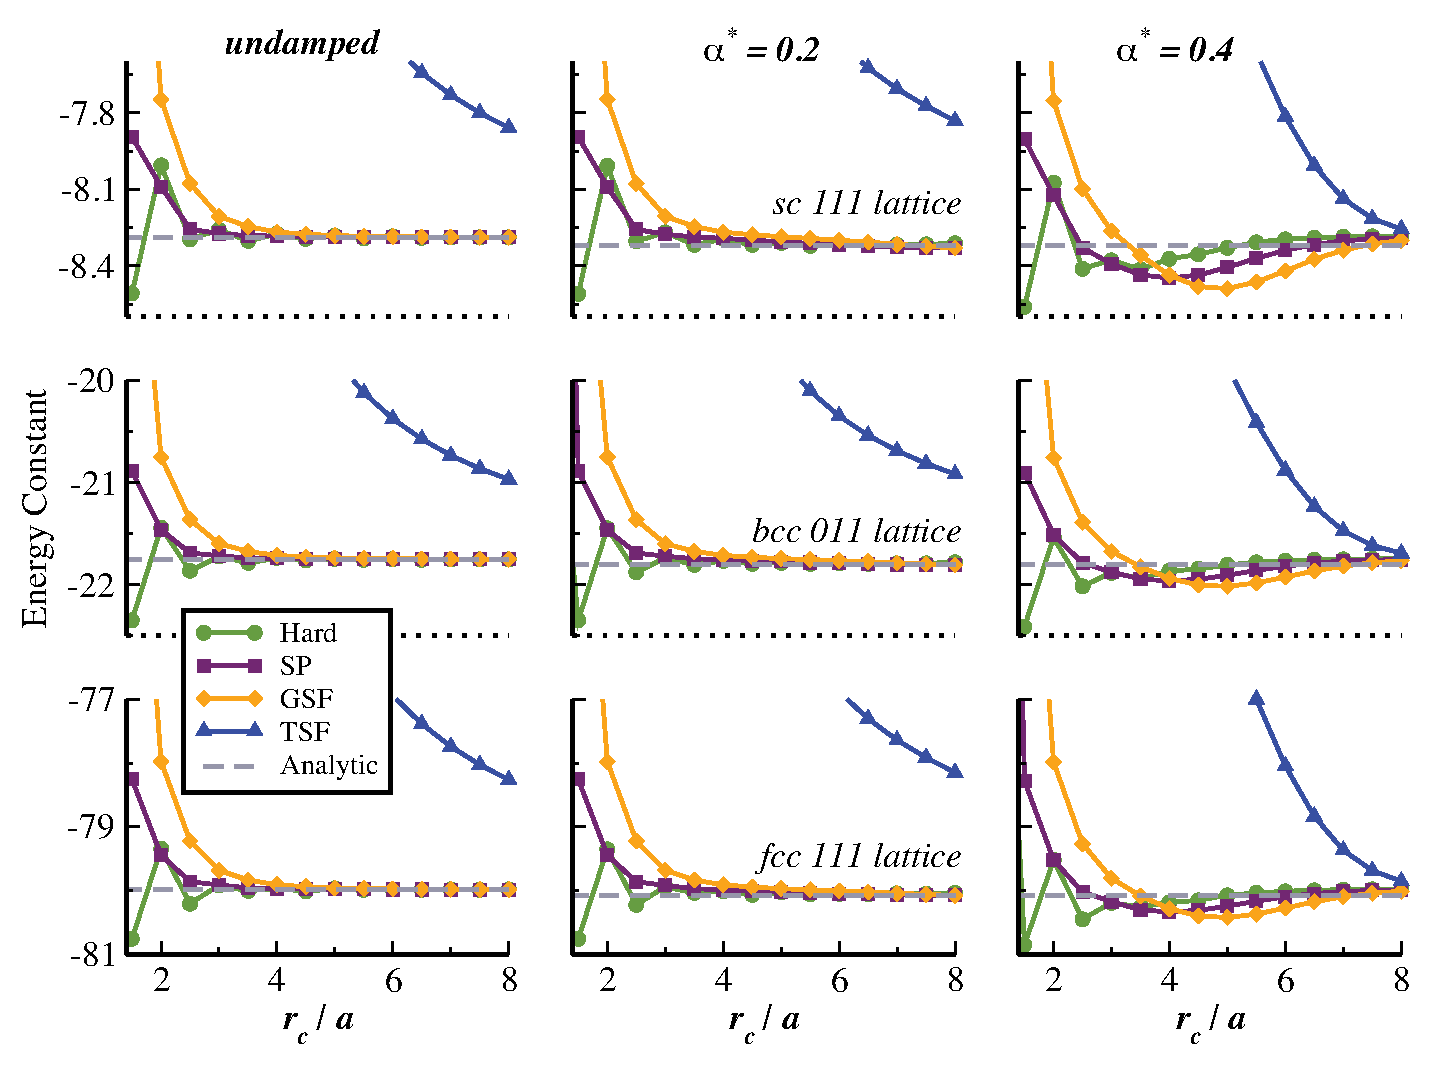
\includegraphics[width=\linewidth]{Quadrupoles_rcut_threeAlpha.eps}
\caption{Convergence of the lattice energy constants as a function of
  cutoff radius (normalized by the lattice constant, $a$) for the new
  real-space methods. Three quadrupolar crystal structures were
  sampled, and the analytic energy constants for the three lattices
  are indicated with grey dashed lines. The left panel shows results
  for the undamped kernel ($1/r$), while the damped kernel, $B_0(r)$
  was used in the center and right panels.  Note that for quadrupoles,
  $\alpha^* = 0.4$ overdamps contributions from repulsive orientations
  in the perfect crystal.}
\label{fig:Quadrupoles_rCut}
\end{figure}

Again, we find that the hard cutoff exhibits oscillations around the
analytic energy constants.  The shifted potential (SP) approximation
converges to the correct energy smoothly by $r_c = 3 a$ even for the
undamped case.  The Taylor-shifted force (TSF) approximation again
appears to perturb the potential too much inside the cutoff region to
provide accurate measures of the energy constants.  GSF again provides
a compromise between the two methods -- energies are converged by $r_c
= 4.5 a$, and the approximation is not as perturbative at short range
as TSF.

It is also useful to understand the behavior of the lattice energy
constants for different values of the reduced damping parameter
($\alpha^* = \alpha a$) for the real-space methods. All of the methods
(except for TSF) have excellent behavior for the undamped or
weakly-damped cases.  Overdamping can cause problems in perfect
crystals for the quadrupoles in particular ({\it cf.} the right panel
in Fig. \ref{fig:Quadrupoles_rCut}). In the perfect crystals, only a
few orientations are being sampled.  E.g. in the simple cubic (SC)
lattice of linear quadrupoles aligned in the 111 direction, the
nearest-neighbor quadrupoles only sample 3 distinct orientations
relative to the vector between the sites.  The damping alters the
radial function for the direct quadrupolar contraction, $v_{41}(r)$,
differently than the radial functions for the terms involving the
product of the separation vector with the quadrupoles, $v_{42}(r)$ and
$v_{43}(r)$.  Because these terms are altered by different amounts by
the complementary error function damping, the effect of damping is
non-spherical for multipoles, and the balance between attractive and
repulsive interactions in the crystal is therefore altered
significantly in overdamped situations.

In the chapter 3, we discuss how large values of
$\alpha$ can perturb the force and torque vectors, but weakly-damped
electrostatics appear to generate reasonable values for the total
electrostatic energies under both the SP and GSF approximations.  We
also discuss the effects that $\alpha$ can have on convergence to the
average electrostatic energies in liquids (which sample a much wider
range of local orientations).

\section{Summary}
We have presented three efficient real-space methods for computing the
interactions between point multipoles.  One of these (SP) is a
multipolar generalization of Wolf's method that smoothly shifts
electrostatic energies to zero at the cutoff radius. Two of these
methods (GSF and TSF) also smoothly truncate the forces and torques
(in addition to the energies) at the cutoff radius, making them
attractive for both molecular dynamics and Monte Carlo simulations. We
find that the Gradient-Shifted Force (GSF) and the Shifted-Potential
(SP) methods converge rapidly to the correct lattice energies for
ordered dipolar and quadrupolar arrays, while the Taylor-Shifted Force
(TSF) is too severe an approximation to provide convergence to lattice
energies within reasonable cutoff radii.

Although the TSF method appears to perform poorly for the analytical
energy constants, the structure of the radial functions used in the
force and torque expressions in the other two methods would not have
been revealed without first developing the TSF approach.  TSF also
generates a set of electrostatic kernels that have multiple
derivatives that vanish at the cutoff radius, a property that is
valuable in estimating dielectric constants using the conducting
boundary fluctuation formula.\cite{Izvekov08}

In most cases, GSF can obtain nearly quantitative agreement with the
lattice energy constants with reasonably small cutoff radii.  The only
exception we have observed is for crystals which exhibit a bulk
macroscopic dipole moment (e.g. Luttinger \& Tisza's $Z_1$ lattice).
In this particular case, the multipole neutralization scheme can
interfere with the correct computation of the energies.  We note that
the energies for these arrangements are typically much larger than for
crystals with net-zero moments, so this is not expected to be an issue
in most simulations.

Relatively weak damping is sufficient to converge to the analytical
energy constants within moderately short cutoff distances. Because
overdamping can present additional issues with higher order
multipoles, our results indicate that the damping coefficient should
be taken as small as possible, and that the {\it undamped} GSF and SP
methods may be the best choice in crystalline systems.

The techniques used here to derive the force, torque and energy
expressions can be extended to higher order multipoles, although some
of the objects (e.g. the matrix cross product in
Eq. \ref{eq:matrixCross}) will need to be generalized for higher-rank
tensors.  We also note that the definitions of the multipoles used
here are in a primitive form, and these need some care when comparing
with experiment or other computational techniques.

In large systems, these new methods can be made to scale approximately
linearly with system size, and detailed comparisons with the Ewald sum
for a wide range of chemical environments follows in the chapter 3.

%
%
%
%
% % uncomment the following lines,
% if using chapter-wise bibliography
%
% \bibliographystyle{ndnatbib}
% \bibliography{example}
